% !TEX encoding = utf8
% !TeX spellcheck = pl_PL


\documentclass[a4paper, 10pt]{article}
\usepackage[utf8]{inputenc}
\usepackage[polish]{babel}
\usepackage{polski}
\usepackage{graphicx}
\usepackage{listings}
\usepackage{amsfonts}
\usepackage{amsmath}
\usepackage{geometry}

\usepackage{float}


\author{Jakub Postępski}
\title{STP - Projekt 2.24}
\graphicspath{{../images/}}
\newgeometry{tmargin=3cm, bmargin=0.5cm, lmargin=0.5cm, rmargin=0.5cm}

\begin{document}
	\maketitle
	Kolejne pliki z katalogu \textit{matlab} odpowiadają zadaniom w kolejnych podsekcjach sprawozdania.
	\section{Wyznaczanie modeli rekurencyjnych}
	Dla podanych danych wyznaczono modele rekurencyjne (tab. \ref{tab:z1}). Na początku przebiegu modele wykazują mniejszy błąd wyjścia. Wizualne obserwacje wyjść modeli potwierdzdają obliczenia błędu. \\
	Wybrano najlepszy model dla $\tau=6$. \\
	Dla najlepszego modelu: $b_6 = -0.1854$, $b_7=-0.918$, $a_1=-1.0403$, $a_2=0.1135$.\\
	Mamy:
	\[y(k)+a_1y(k-1) + a_2y(k-2)=b_6u(k-6)+b_7u(k-7)\]
	Po zastosowaniu transformaty $Z$:
	\[(1+a_1z^{-1} + a_2z^{-2})Y(z)=(b_6z^{-6}+b_7z^{-7})U(z)\]
	Więc transmitancja:
	\[G(z)=\frac{Y(z)}{U(z)}=\frac{b_6z^{-6}+b_7z^{-7}}{1+a_1z^{-1} + a_2z^{-2}}=\frac{-0.1854z^{-6}-0.918z^{-7}}{1-1.0403z^{-1} + 0.1135z^{-2}}\]
	\begin{table}[H]
	\centering
	\begin{tabular}{|c|c|c|c|c|c|c|}
	\hline 
	$\tau$ & $b_\tau$ & $b_{\tau+1}$ & $-a_1$ & $-a_2$ & $E$ & rys. \\ 
	\hline 
	 1 & -0.0082 & -0.0679 &  1.6619 & -0.6799
	  & 79.2282 & \ref{fig:z1_1}\\ 
	\hline 
	2 & 0.0027 & -0.1003
	  &  1.5901 & -0.6135 & 54.2224 & \ref{fig:z1_2}\\ 
	\hline 3 & -0.0014 & -0.1337 &  1.4685  & -0.5010 & 39.9572 & \ref{fig:z1_3}\\ 
	\hline 
	4 & -0.0568 & -0.1271 & 1.3107 & -0.3552
	  & 32.3080  & \ref{fig:z1_4}\\ 
	\hline 
 5 & -0.1188 & -0.1281 & 1.1146 &  -0.1763 & 20.9694 & \ref{fig:z1_5} \\ 
	\hline 
	6 & -0.1854  &  -0.0918 &  1.0403  & -0.1135 & 16.3988 &\ref{fig:z1_6} \\ 
	\hline 
	7 & -0.1575 & -0.0517  & 1.2836 & -0.3445  & 46.8691
	&\ref{fig:z1_7} \\ 
	\hline
	8 & -0.1146 & 0.0001  & 1.5764 & -0.6144 & 176.8823 & \ref{fig:z1_8} \\ 
	\hline 
	\end{tabular}
	\label{tab:z1}
	\caption{Porównanie modeli rekurencyjnych}
	\end{table}
	
	\begin{figure}[H]
	\centering
	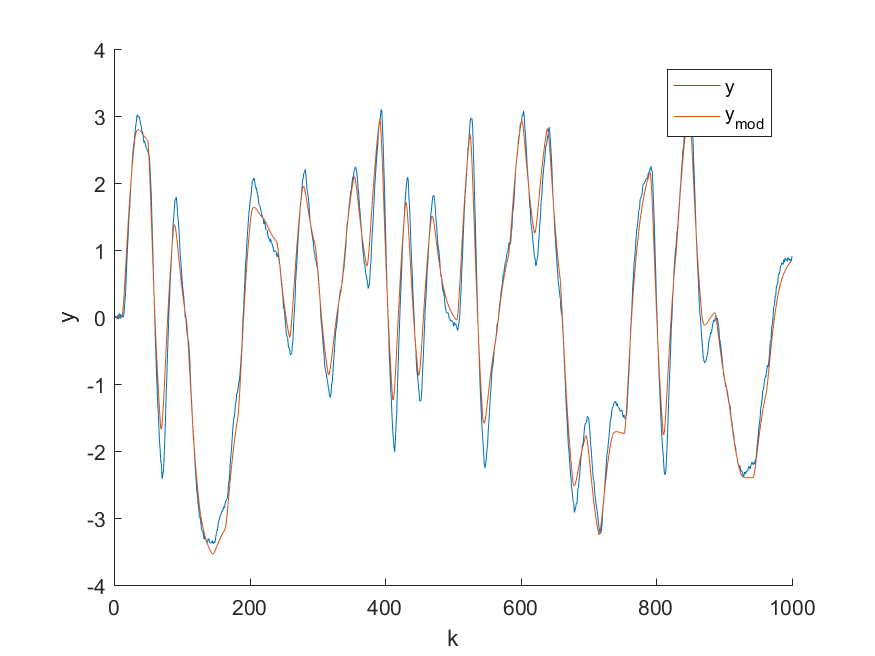
\includegraphics[width=0.9\linewidth]{z1_1}
	\caption{Wyjścia modelu dla $\tau=1$}
	\label{fig:z1_1}
	\end{figure}
	\begin{figure}[H]
	\centering
	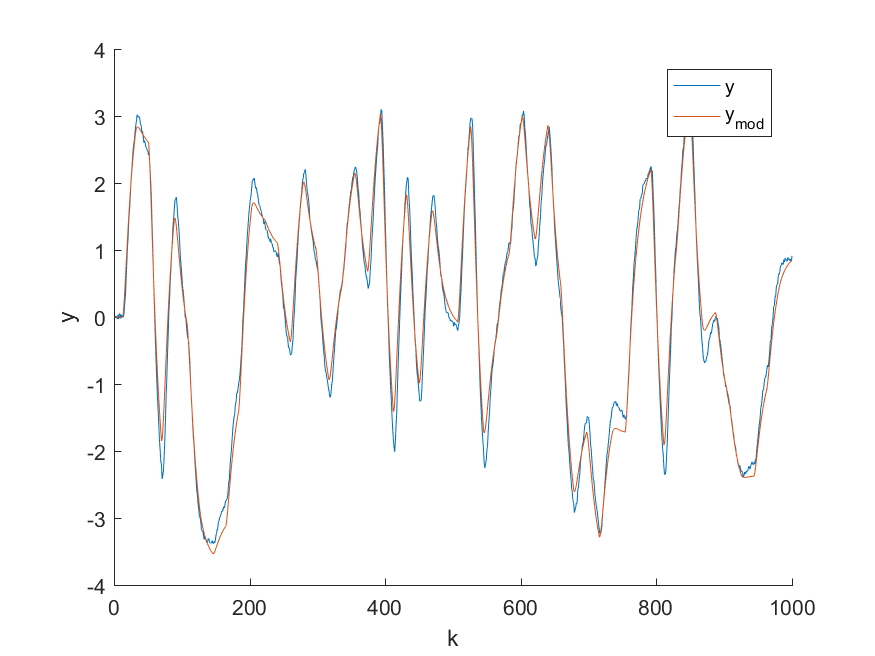
\includegraphics[width=0.9\linewidth]{z1_2}
	\caption{Wyjścia modelu dla $\tau=2$}
	\label{fig:z1_2}
	\end{figure}
	\begin{figure}[H]
	\centering
	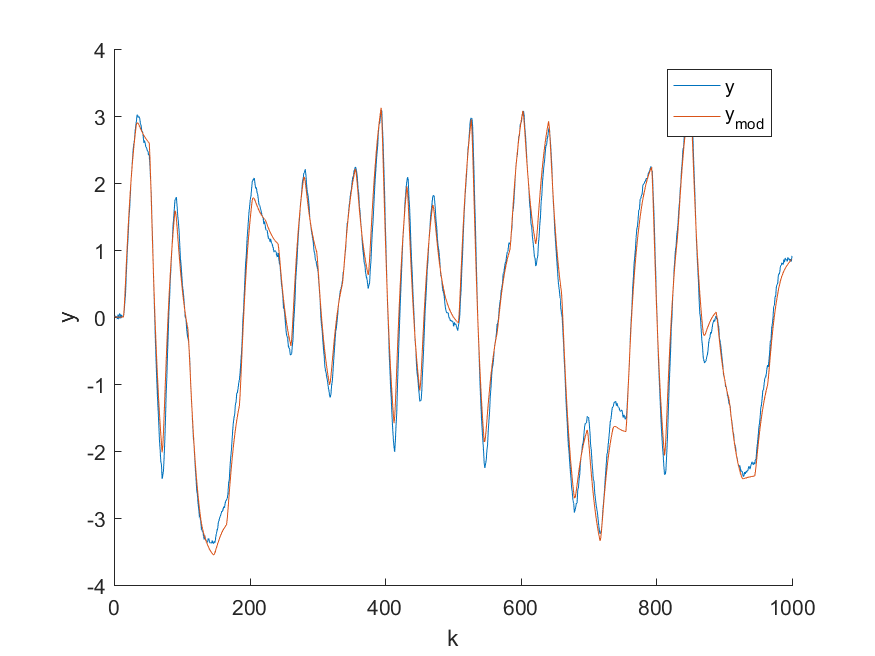
\includegraphics[width=0.9\linewidth]{z1_3}
	\caption{Wyjścia modelu dla $\tau=3$}
	\label{fig:z1_3}
	\end{figure}
	\begin{figure}[H]
	\centering
	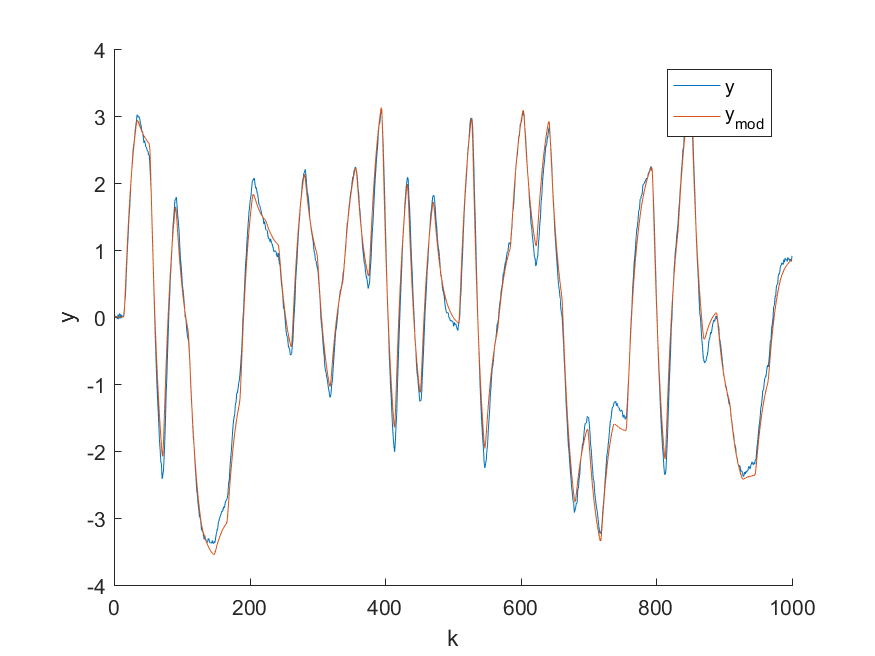
\includegraphics[width=0.9\linewidth]{z1_4}
	\caption{Wyjścia modelu dla $\tau=4$}
	\label{fig:z1_4}
	\end{figure}
	\begin{figure}[H]
	\centering
	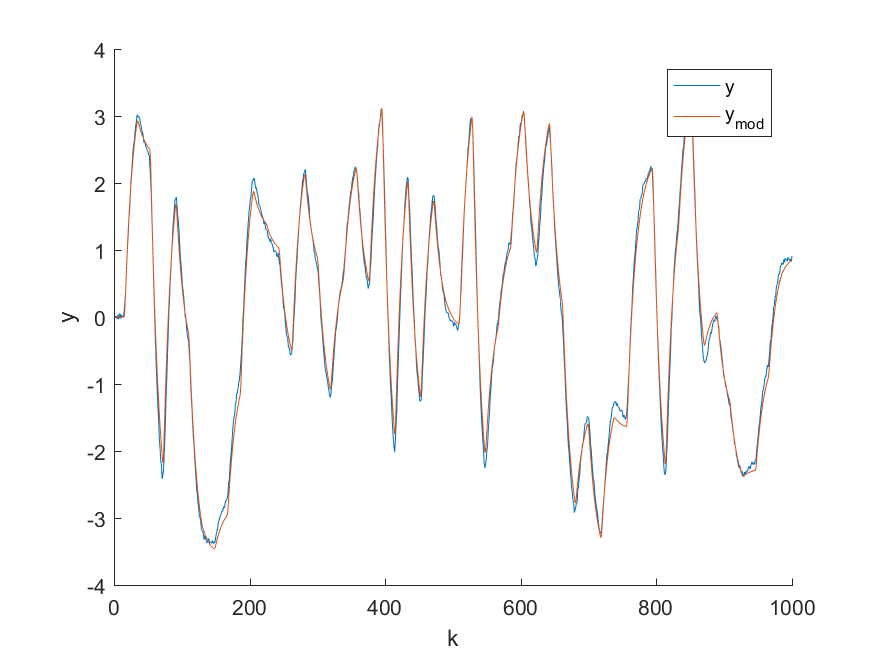
\includegraphics[width=0.9\linewidth]{z1_5}
	\caption{Wyjścia modelu dla $\tau=5$}
	\label{fig:z1_5}
	\end{figure}
	\begin{figure}[H]
	\centering
	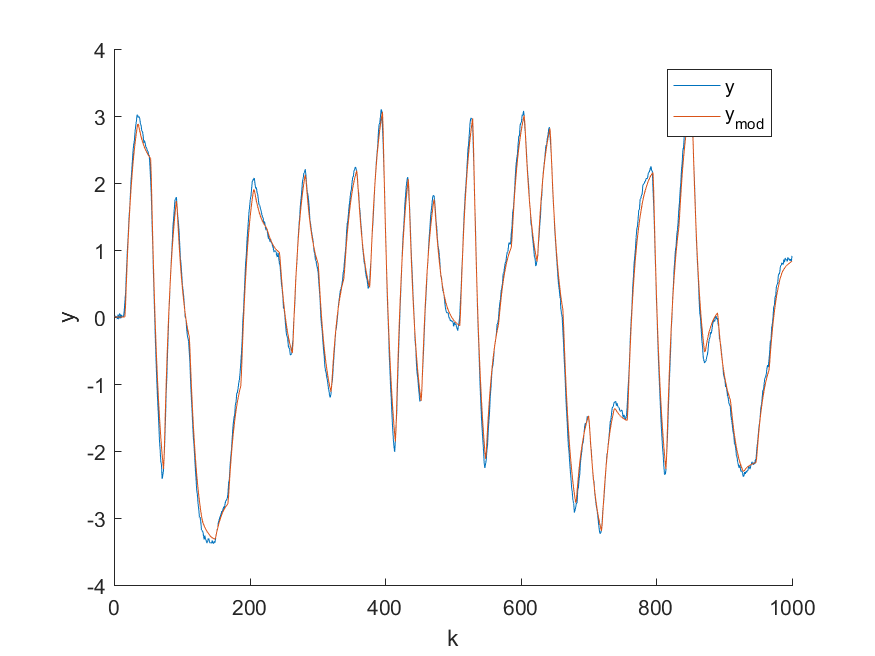
\includegraphics[width=0.9\linewidth]{z1_6}
	\caption{Wyjścia modelu dla $\tau=6$}
	\label{fig:z1_6}
	\end{figure}
	\begin{figure}[H]
	\centering
	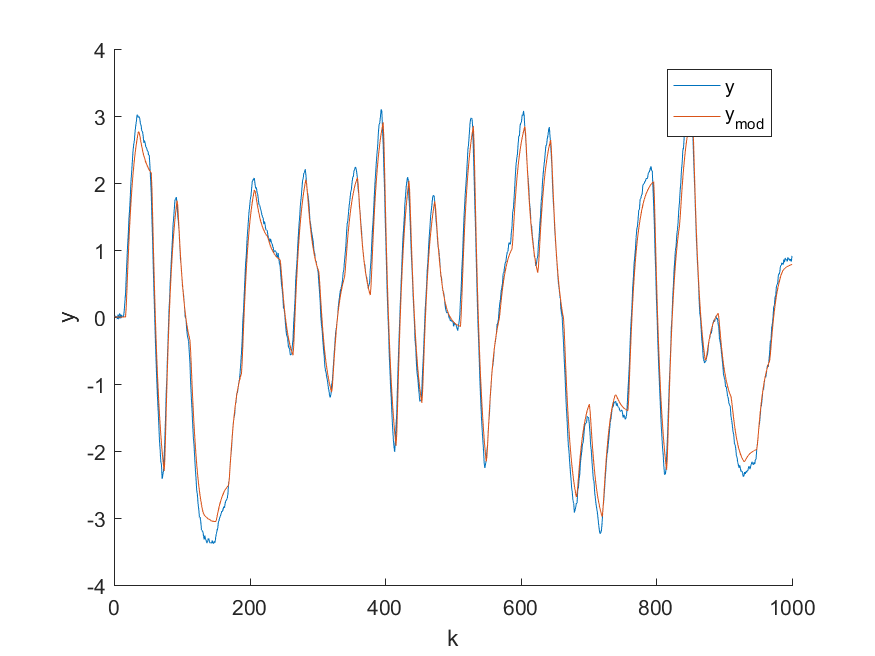
\includegraphics[width=0.9\linewidth]{z1_7}
	\caption{Wyjścia modelu dla $\tau=7$}
	\label{fig:z1_7}
	\end{figure}
	\begin{figure}[H]
	\centering
	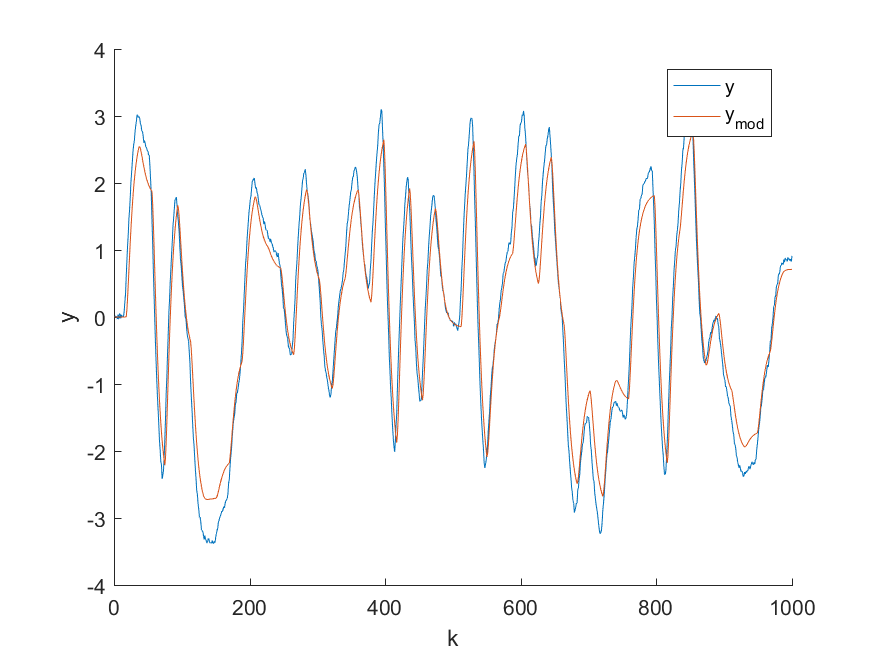
\includegraphics[width=0.9\linewidth]{z1_8}
	\caption{Wyjścia modelu dla $\tau=8$}
	\label{fig:z1_8}
	\end{figure}

	\section{Odpowiedz skokowa}
	Obliczono ze wzoru odpowiedz skokową (rys. \ref{fig:z2}).\\
	Wzmocnienie statyczne:
	\[K_{stat}=\lim_{z\rightarrow 1}G(z)=-3.7848\]
	\begin{figure}[H]
		\centering
		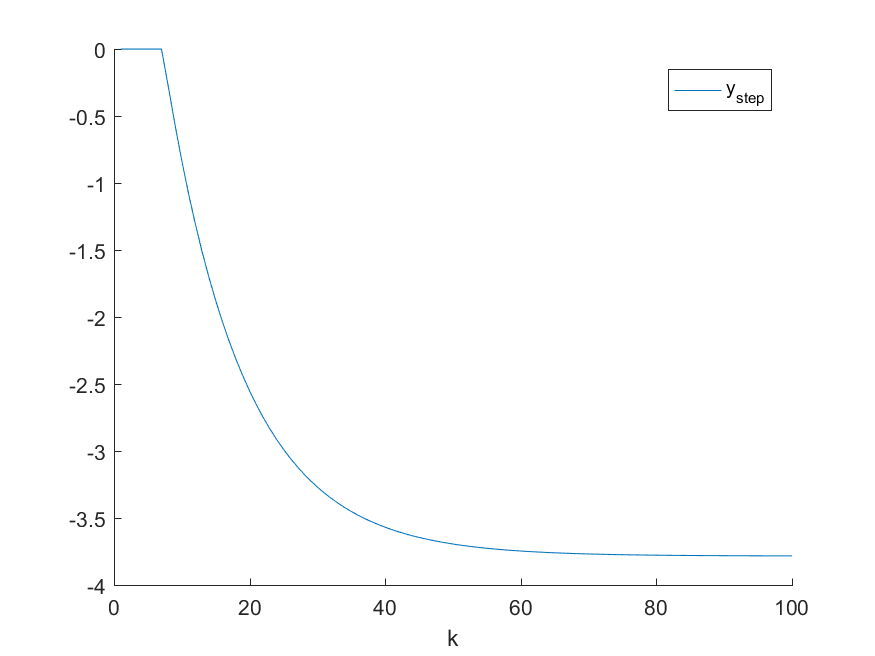
\includegraphics[width=0.9\linewidth]{z2}
		\caption{Odpowiedz skokowa modelu}
		\label{fig:z2}
		\end{figure}
		
	\section{Regulator PID}
	Dla regulatora postaci:
	\[G_r(z)=\frac{u(k)}{e(k)} = \frac{r_2z^{-2}+r_1z^{-1}+r_0}{1-z^{-1}}\]
	Mamy:
	\[r_2=K\frac{T_d}{T}\]
	\[r_1=K(\frac{T}{2T_i}-2\frac{T_d}{T}-1)\]
	\[r_0=K(1+\frac{T}{2T_i}+\frac{T_d}{T})\]
	
	Zgodnie z eksperymentem Zieglera-Nicholsa:
	\[K_k = \]
	\[T_k = \]
	\[K = 0.6K_k = \]
	\[T_i = 0.5T_k = \]
	\[T_d = 0.12T_k = \]
	
	\section{Regulator DMC}
	\subsection{Strojenie nastawów}
	Przyjęto $Y_{zad}=5$. Dla podpunktów a) do d) dobrano regulator ($D=70$, $N=20$, $N_u=6$, $\lambda=1$) o odpowiednio małych horyzontach niepogarszających regulacji (rys. \ref{fig:z4_1}). Uzyskano $J_y=4.23$ oraz $J_y = 184.99$.
	
	\begin{figure}[H]
			\centering
			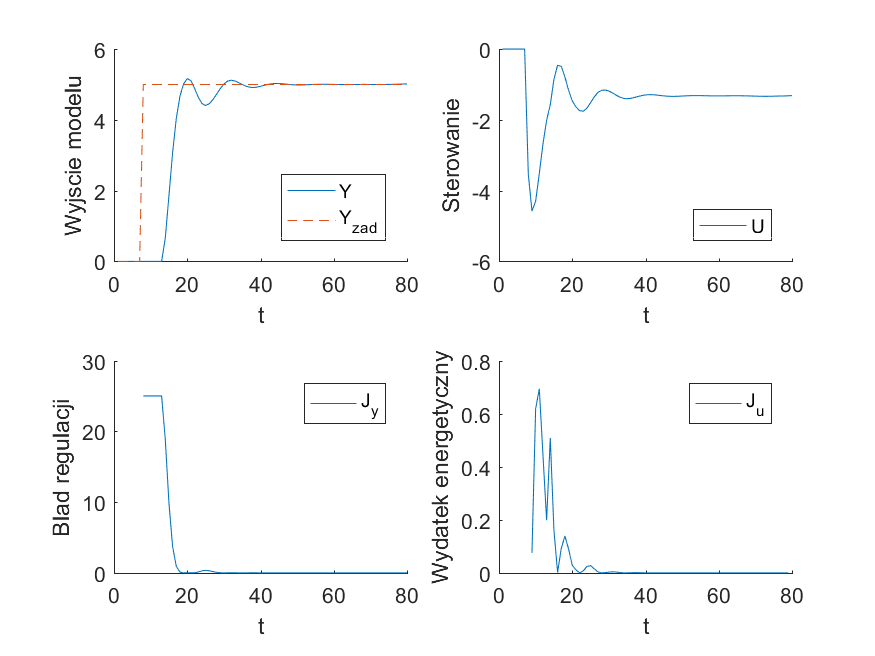
\includegraphics[width=0.9\linewidth]{z4_70_20_6_1}
			\caption{Symulacja regulacji dla $D=70$, $N=20$, $N_u=6$, $\lambda=1$}
			\label{fig:z4_1}
			\end{figure}
			
	Przy zmniejszaniu wartości parametru $\lambda$ uzyskiwano gorszej jakości wyjście modelu (większe oscylacje) oraz mniejsze zmiany sterowania (np. $J_y=5.60$, $J_u=180.31$ dla symulacji z rys. \ref{fig:z4_2})
	
	\begin{figure}[H]
				\centering
				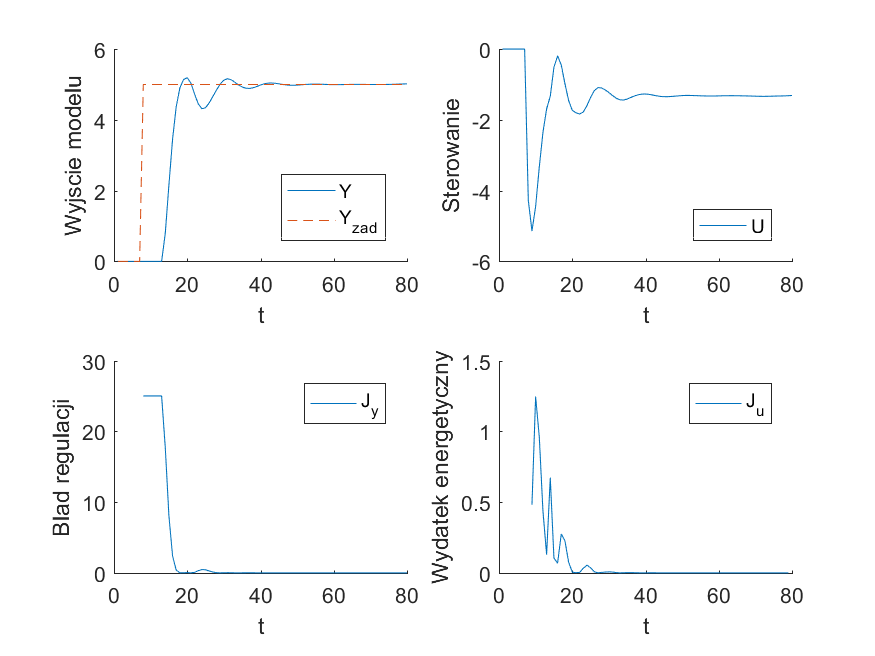
\includegraphics[width=0.9\linewidth]{z4_70_20_6_06}
				\caption{Symulacja regulacji dla $D=70$, $N=20$, $N_u=6$, $\lambda=0.6$}
				\label{fig:z4_2}
				\end{figure}
				
	Przy zwiększaniu wartości parametru $\lambda$ uzyskiwano lepszej jakości wyjście modelu (mniejsze oscylacje, brak przeregulowania) i wejście o większych zmianach (np. $J_y=1.63$, $J_u=210.50$ dla symulacji z rys. \ref{fig:z4_3}
	
		\begin{figure}[H]
					\centering
					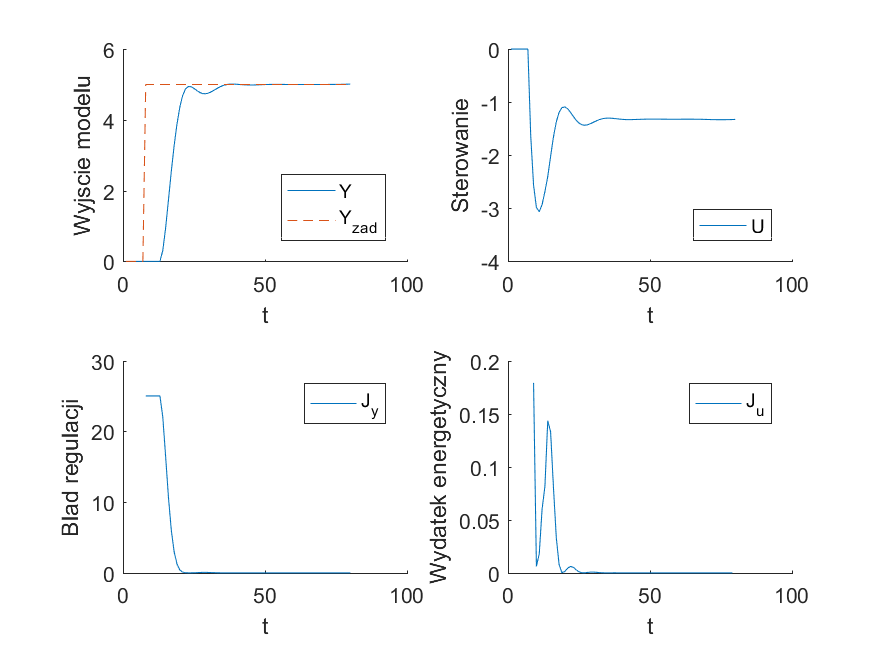
\includegraphics[width=0.9\linewidth]{z4_70_20_6_6}
					\caption{Symulacja regulacji dla $D=70$, $N=20$, $N_u=6$, $\lambda=6$}
					\label{fig:z4_3}
					\end{figure}
					
	Ostatecznie ustalono optymalne nastawy dla $\lambda = 3$ ($J_y=2.43$, $J_u=198.40$, rys. \ref{fig:z4_4}).
	
	\begin{figure}[H]
				\centering
				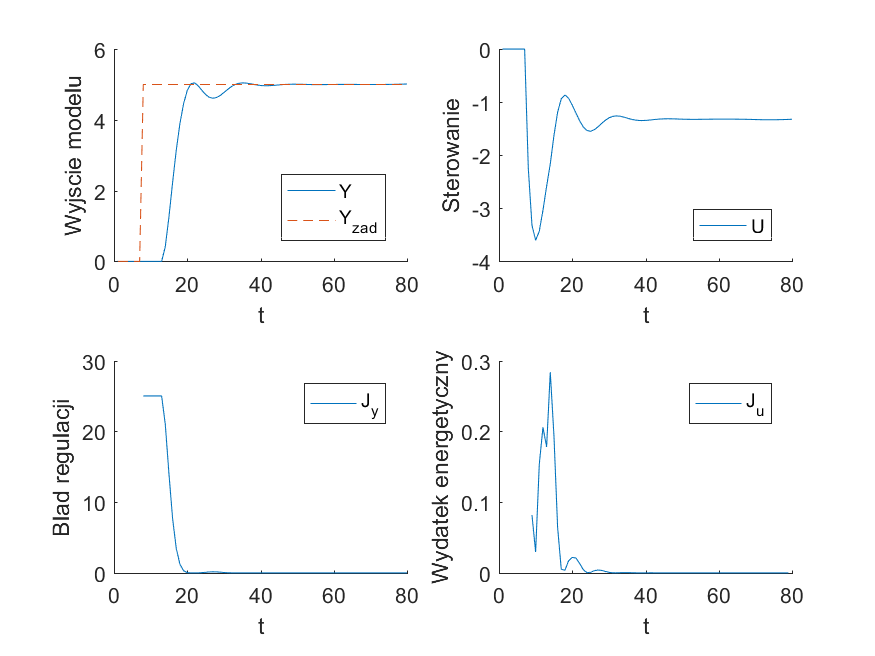
\includegraphics[width=0.9\linewidth]{z4_70_20_6_3}
				\caption{Symulacja regulacji dla $D=70$, $N=20$, $N_u=6$, $\lambda=3$}
				\label{fig:z4_4}
				\end{figure}
				
	\subsection{Niemierzalne zakłócenie wyjścia}
	Do wyjścia modelu dodano zakłócenie wartości $Y_{szum} = 1$ od chwili $T=40$ (rys. \ref{fig:z5}). Spowodowało to zmianę w sterowaniu modelem przez regulator i zmianę w przebiegu wyjścia modelu lecz ostatecznie poprawną regulację. Nawet podczas dalszego zwiększania (np. $Y_{szum}=6$, rys. \ref{fig:z56}) obiekt był regulowany poprawnie, co spowodowane wykorzystaniem różnic poprzednich sterowań w regulatorze.
	
		\begin{figure}[H]
		\centering
		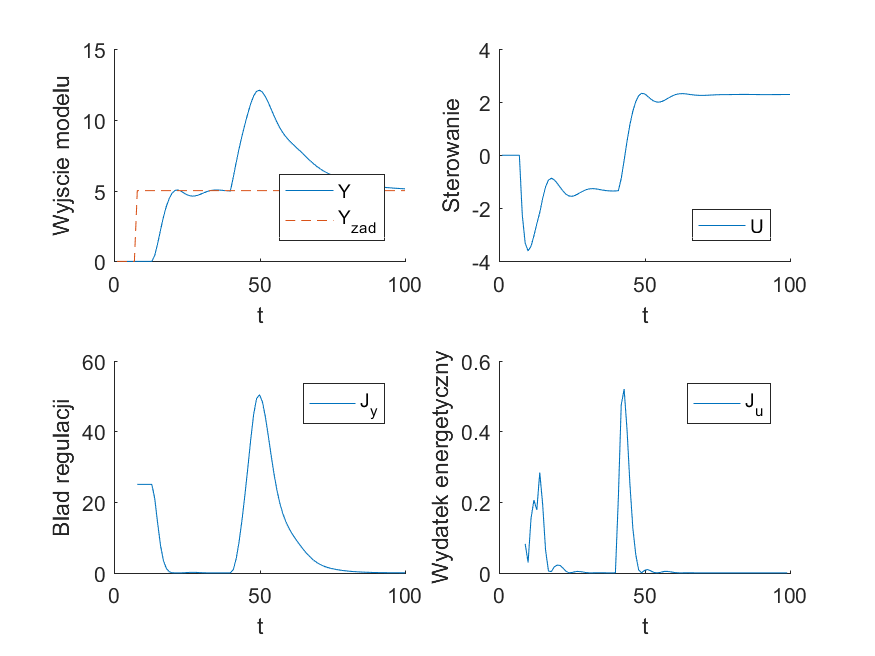
\includegraphics[width=0.9\linewidth]{z5}
		\caption{Symulacja regulacji z niemierzalnym zakłóceniem wartości $1$.}
		\label{fig:z5}
		\end{figure} 
			\begin{figure}[H]
				\centering
				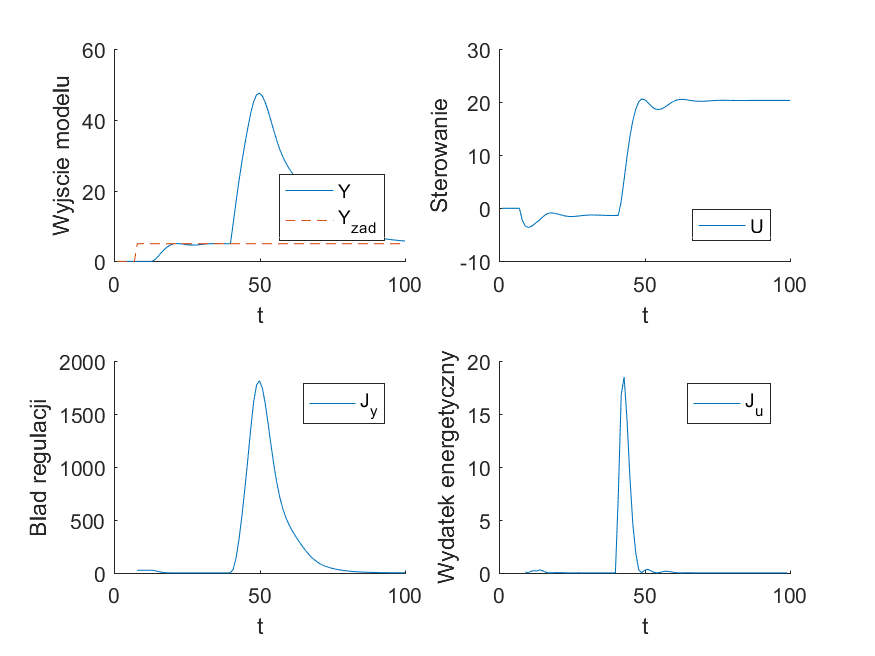
\includegraphics[width=0.9\linewidth]{z56}
				\caption{Symulacja regulacji z niemierzalnym zakłóceniem wartości $6$.}
				\label{fig:z56}
				\end{figure} 
				
				
	\subsection{Testowanie odporności}
	Przyjęto w/w przyjęte parametry regulacji. Dla zmniejszonego czasu odpowiedzi występują oscylacje wejścia i wyjścia modelu (rys. \ref{fig:z6_1}, rys.\ref{fig:z6_3}, rys.\ref{fig:z6_5}). Dla zwiększonego czasu odpowiedzi występują oscylację sygnału wejściowego i pogorszenie regulacji (rys. \ref{fig:z6_-1}, \ref{fig:z6_-3}, \ref{fig:z6_-10}). Dla opóźnień oraz małych przyspieszeń inercji obiektu udaje się uzyskać regulację.
	\begin{figure}[H]
	\centering
	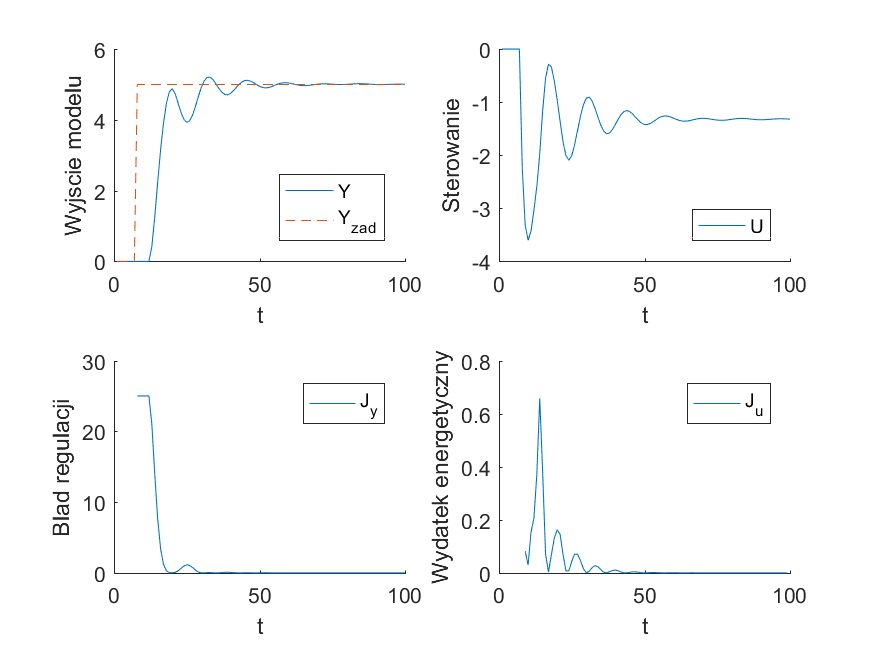
\includegraphics[width=0.9\linewidth]{z6_1}
	\caption{Testowanie odporności dla  $y(k) = b_6u(k-5)+b_7u(k-6)-a_1y(k-1)-a_2y(k-2)=$.}
	\label{fig:z6_1}
	\end{figure}
	
	\begin{figure}[H]
		\centering
		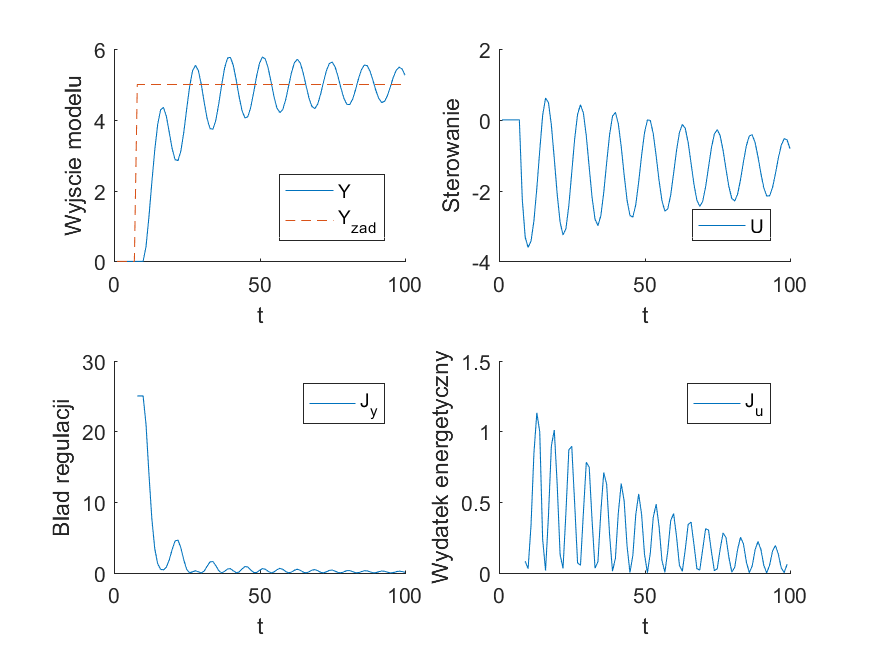
\includegraphics[width=0.9\linewidth]{z6_3}
		\caption{Testowanie odporności dla  $y(k) = b_6u(k-3)+b_7u(k-4)-a_1y(k-1)-a_2y(k-2)$.}
		\label{fig:z6_3}
		\end{figure}
		
	\begin{figure}[H]
			\centering
			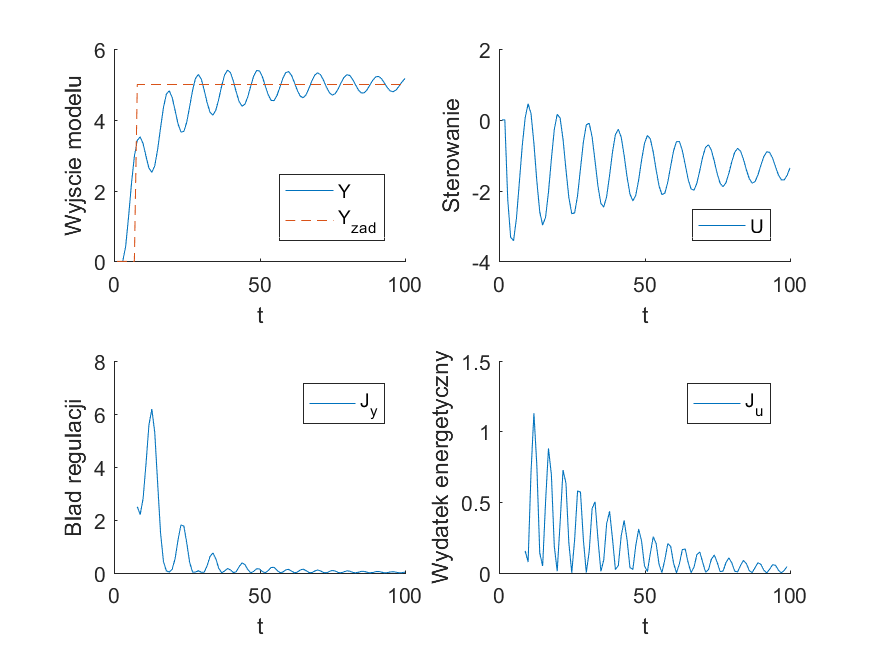
\includegraphics[width=0.9\linewidth]{z6_5}
			\caption{Testowanie odporności dla  $y(k) = b_6u(k-1)+b_7u(k-2)-a_1y(k-1)-a_2y(k-2)$.}
			\label{fig:z6_5}
			\end{figure}
		
	\begin{figure}[H]
		\centering
		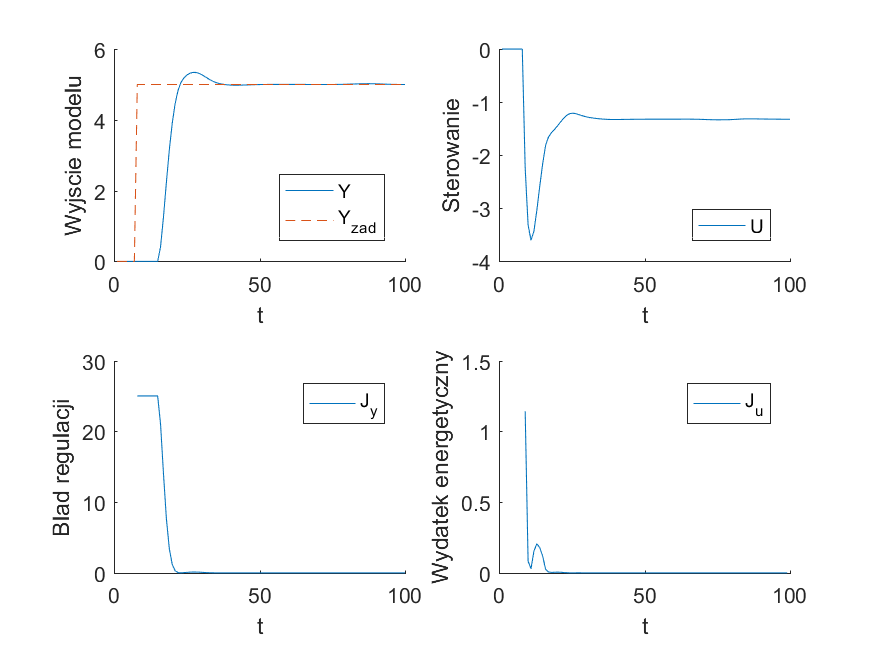
\includegraphics[width=0.9\linewidth]{z6_-1}
		\caption{Testowanie odporności dla  $y(k) = b_6u(k-7)+b_7u(k-8)-a_1y(k-1)-a_2y(k-2)$.}
		\label{fig:z6_-1}
		\end{figure}
		
	\begin{figure}[H]
		\centering
		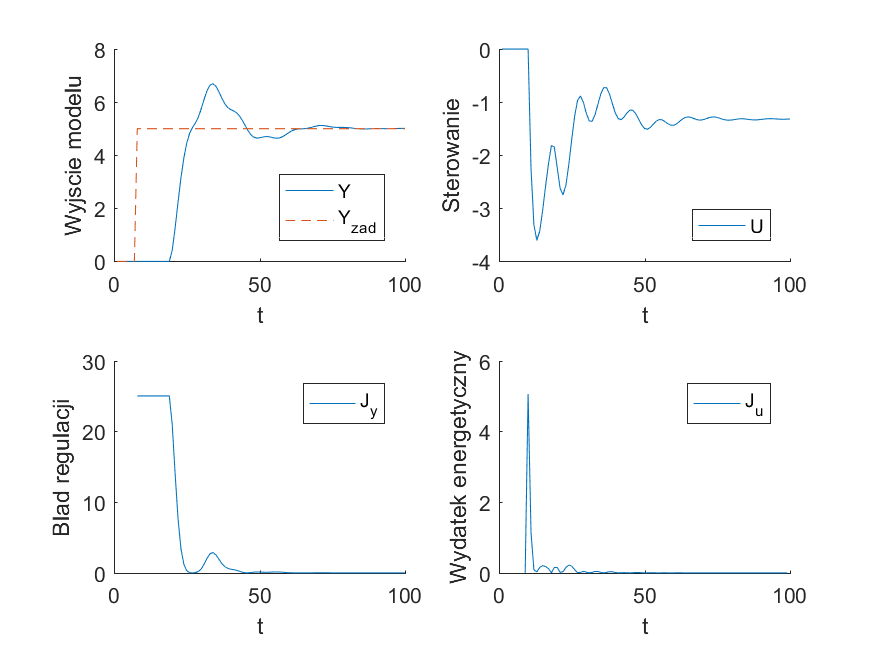
\includegraphics[width=0.9\linewidth]{z6_-3}
		\caption{Testowanie odporności dla  $y(k) = b_6u(k-9)+b_7u(k-10)-a_1y(k-1)-a_2y(k-2)$.}
		\label{fig:z6_-3}
		\end{figure}
		
	\begin{figure}[H]
			\centering
			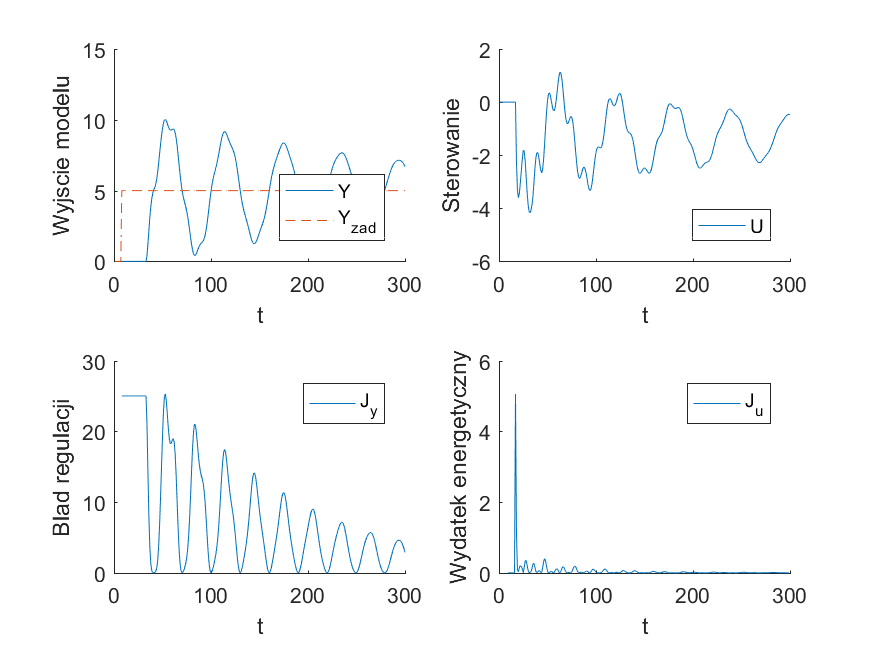
\includegraphics[width=0.9\linewidth]{z6_-10}
			\caption{Testowanie odporności dla  $y(k) = b_6u(k-16)+b_7u(k-17)-a_1y(k-1)-a_2y(k-2)$.}
			\label{fig:z6_-10}
			\end{figure}
	
	\subsection{Ograniczenia wartości i zmiany sygnału sterującego}
	Dla wyżej przyjętych optymalnych parametrów regulacji:
	\begin{itemize}
	\item Dla ograniczeń wyłączenie wartości nie zawsze udaje się osiągnąć regulację (np. rys. \ref{fig:z7_200_-1_1}) lub regulacja jest wolniejsza (np. rys. \ref{fig:z7_200_-2_0}). Może nastąpić zmniejszenie wydatku energetycznego. $J_u$. Zmniejszenie stabilności.
	
	\item Dla ograniczeń wyłącznie zmiany synału sterującego większe przeregulowanie (np. rys. \ref{fig:z7_1_-1000_100}). W skrajnych przypadkach brak regulacji, oscylacje wejścia i wyjścia (np. rys. \ref{fig:z7_01_-1000_100}). Zmniejszenie szybkości regulacji i reagowania na zmiany. 
	
	\item  Najlepszy przebieg otrzymujemy bez wprowadzania ograniczeń (rys. \ref{fig:z4_4}).
	\end{itemize}
	
	\begin{figure}[H]
				\centering
				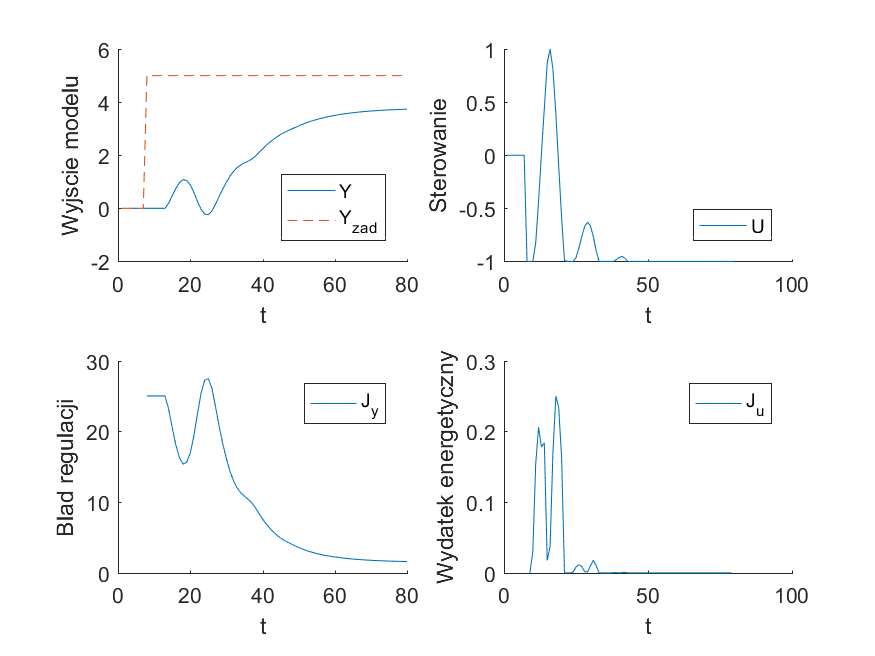
\includegraphics[width=0.9\linewidth]{z7_200_-1_1}
				\caption{Ogranicznenie  $-1<u(k)<1$}
				\label{fig:z7_200_-1_1}
				\end{figure}
	\begin{figure}[H]
				\centering
				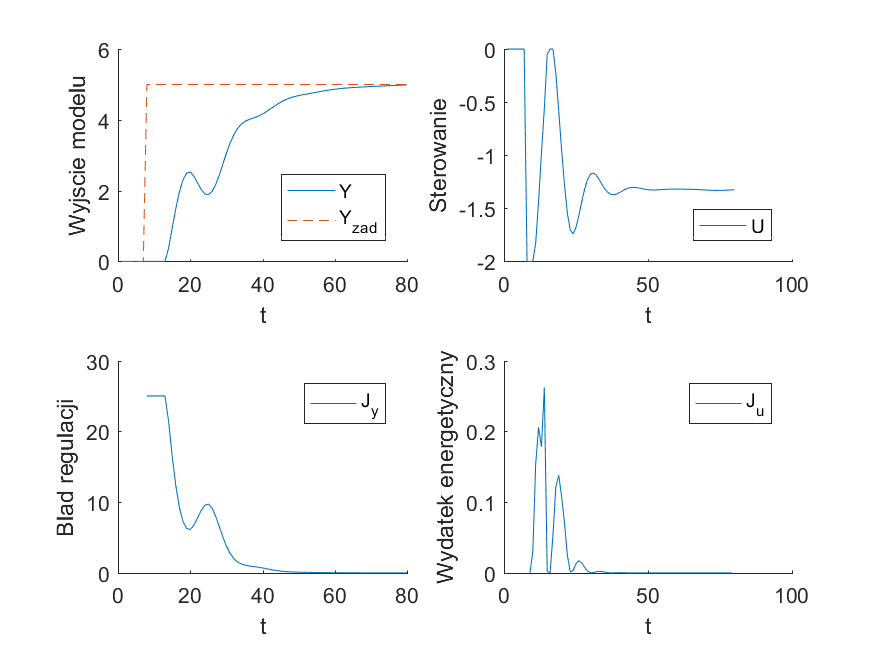
\includegraphics[width=0.9\linewidth]{z7_200_-2_0}
				\caption{Ograniczenie $-2<u(k)<0$}
				\label{fig:z7_200_-2_0}
				\end{figure}
	
	\begin{figure}[H]
					\centering
					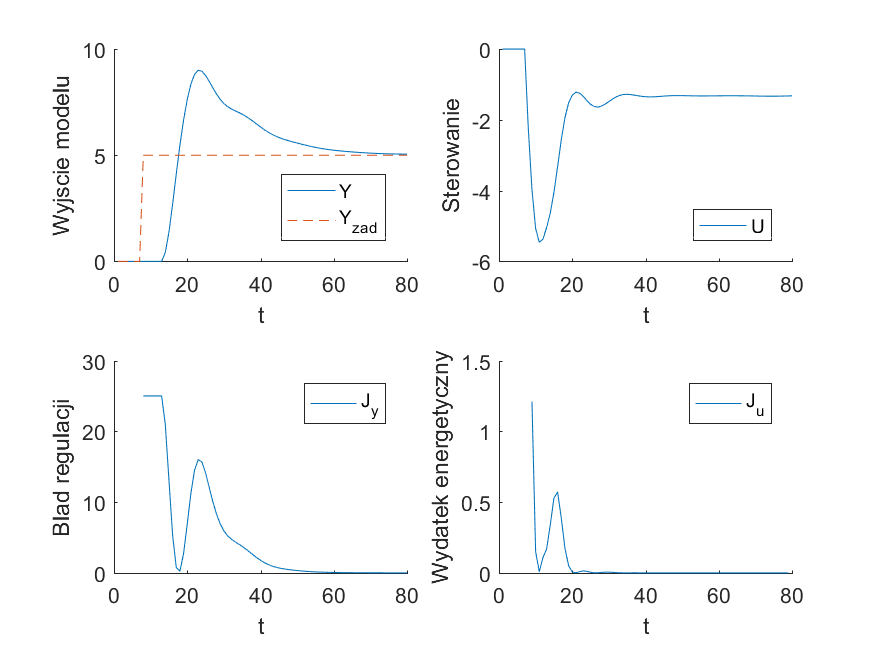
\includegraphics[width=0.9\linewidth]{z7_1_-1000_100}
					\caption{Ograniczenie $\Delta u < 1$}
					\label{fig:z7_1_-1000_100}
					\end{figure}
	\begin{figure}[H]
				\centering
				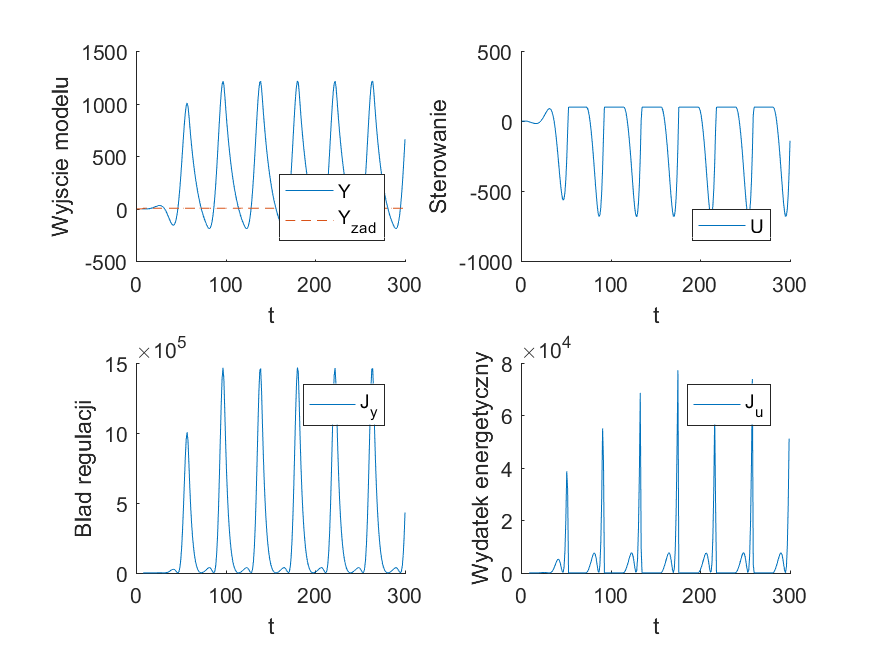
\includegraphics[width=0.9\linewidth]{z7_01_-1000_100}
				\caption{Ogranicznenie  $\Delta u < 0.1$}
				\label{fig:z7_01_-1000_100}
				\end{figure}	
\end{document}